\documentclass[12pt]{article}%
\usepackage{graphicx}
\usepackage{subfig}
\usepackage[font=small,labelfont=bf]{caption}
\usepackage{hyperref} 

\usepackage[style=verbose]{biblatex}

\usepackage{filecontents}% to embed the file `myreferences.bib` in your `.tex` file

\begin{filecontents}{myreferences.bib}
@online{foo12,
  year = {2012},
  title = {footnote-reference-using-european-system},
  url = {http://tex.stackexchange.com/questions/69716/footnote-reference-using-european-system},
}
\end{filecontents}

% File is created and written to disk by the above package
\addbibresource{myreferences.bib}


\begin{document}

\title{Identifying Fraud at Enron Data}
\author{Badrinath Thirumalachari}
\date{\today}
\maketitle 
 

\section*{Introduction}

Enron Corporation was an American energy, commodities, and services company based in Houston, Texas. It was founded in 1985 as the result of a merger between Houston Natural Gas and InterNorth, both relatively small regional companies in the U.S. Before its bankruptcy on December 2, 2001, Enron employed approximately 20,000 staff and was one of the world's major electricity, natural gas, communications and pulp and paper companies, with claimed revenues of nearly \$101 billion during 2000.\footcite{https://en.wikipedia.org/wiki/Enron}
\\
At the end of 2001, it was revealed that its reported financial condition was sustained by institutionalized, systematic, and creatively planned accounting fraud, known since as the Enron scandal. Enron has since become a well-known example of willful corporate fraud and corruption. The data relevant to this scandal was made public. This dataset was collected and prepared by the CALO Project (A Cognitive Assistant that Learns and Organizes). It contains data from about 150 users, mostly senior management of Enron, organized into folders.\footcite{https://en.wikipedia.org/wiki/Enron}
\\
The goal of this project is to use predictive machine learning models correctly predict persons of interest (POI) who were individuals who were involved in this scandal, using financial compensation data and aggregate email statistics from the Enron Corpus.
\printbibliography
\newpage
\section*{Question 1}

Summarize for us the goal of this project and how machine learning is useful in trying to accomplish it. As part of your answer, give some background on the dataset and how it can be used to answer the project question. Were there any outliers in the data when you got it, and how did you handle those?

\subsection*{Solution}

The data contained 146 total records with 18 people labeled as POI's. After looking through the data in detail, a few outliers were found and removed. 	

\subsubsection*{Outliers}

Glancing through the data and investigating it deeply outliers were found in keys 'TOTAL' and 'THE TRAVEL AGENCY IN THE PARK'. These outliers were removed before feature creation.

\begin{figure}[!htbp]
  \centering
  \subfloat[Data with outlier]{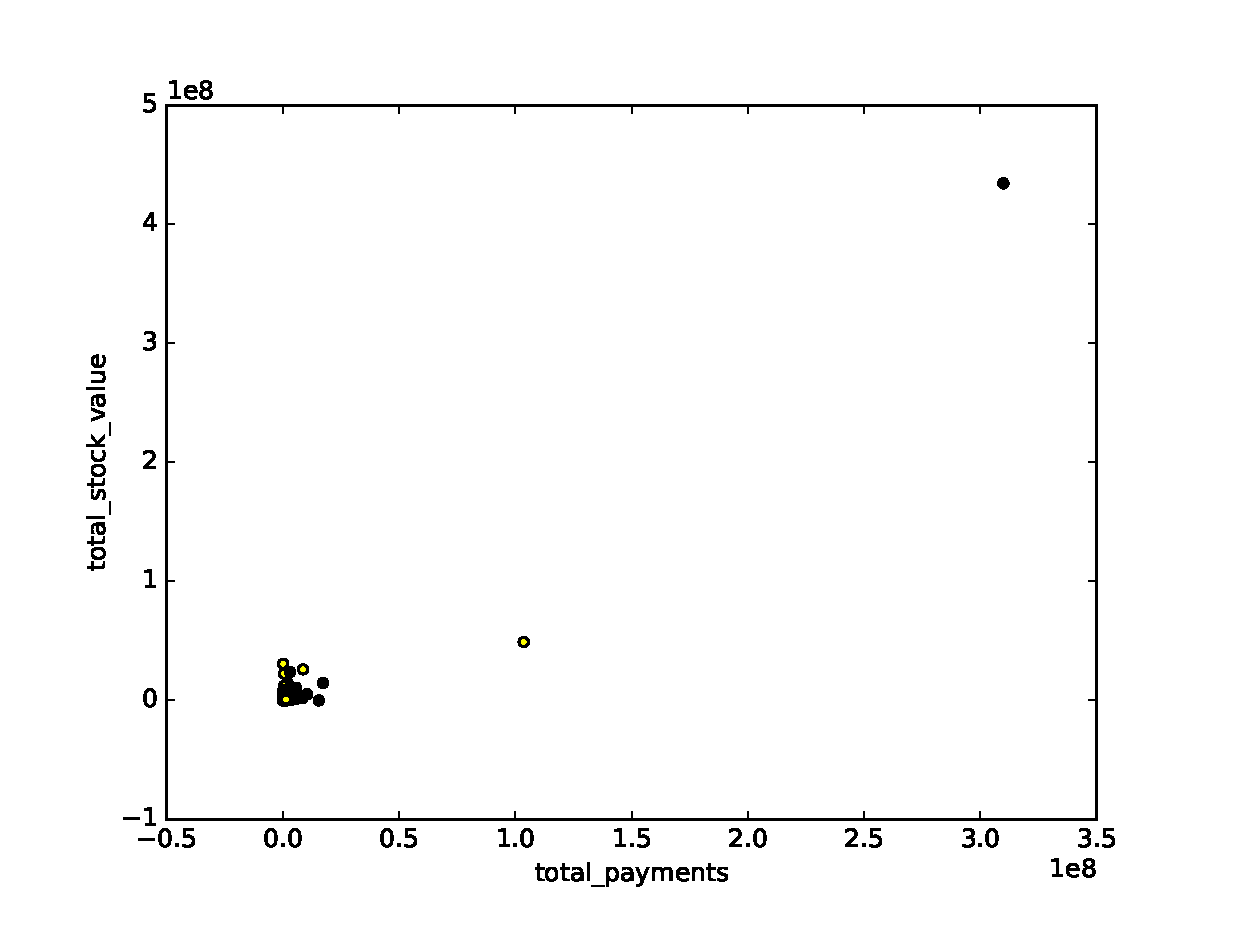
\includegraphics[width=1\textwidth]{outlier1.eps}}
  \hfill
  \subfloat[Data after outlier removal]{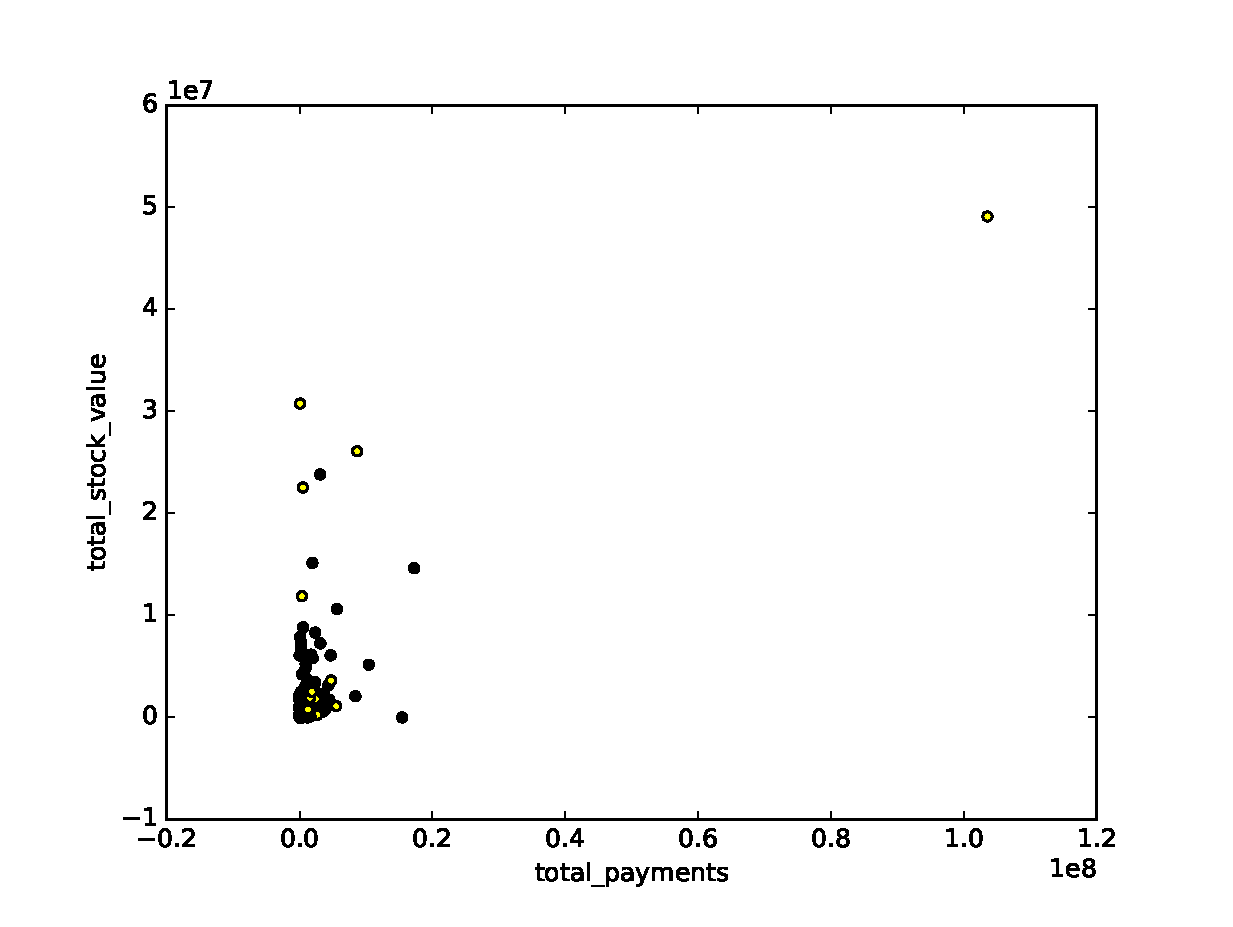
\includegraphics[width=1\textwidth]{notoutlier1.eps}}
  \caption{Total payments vs total stock value, POI's are marked in yellow}
\end{figure}


\begin{figure}[!htbp]
  \centering
  \subfloat[Data with outlier]{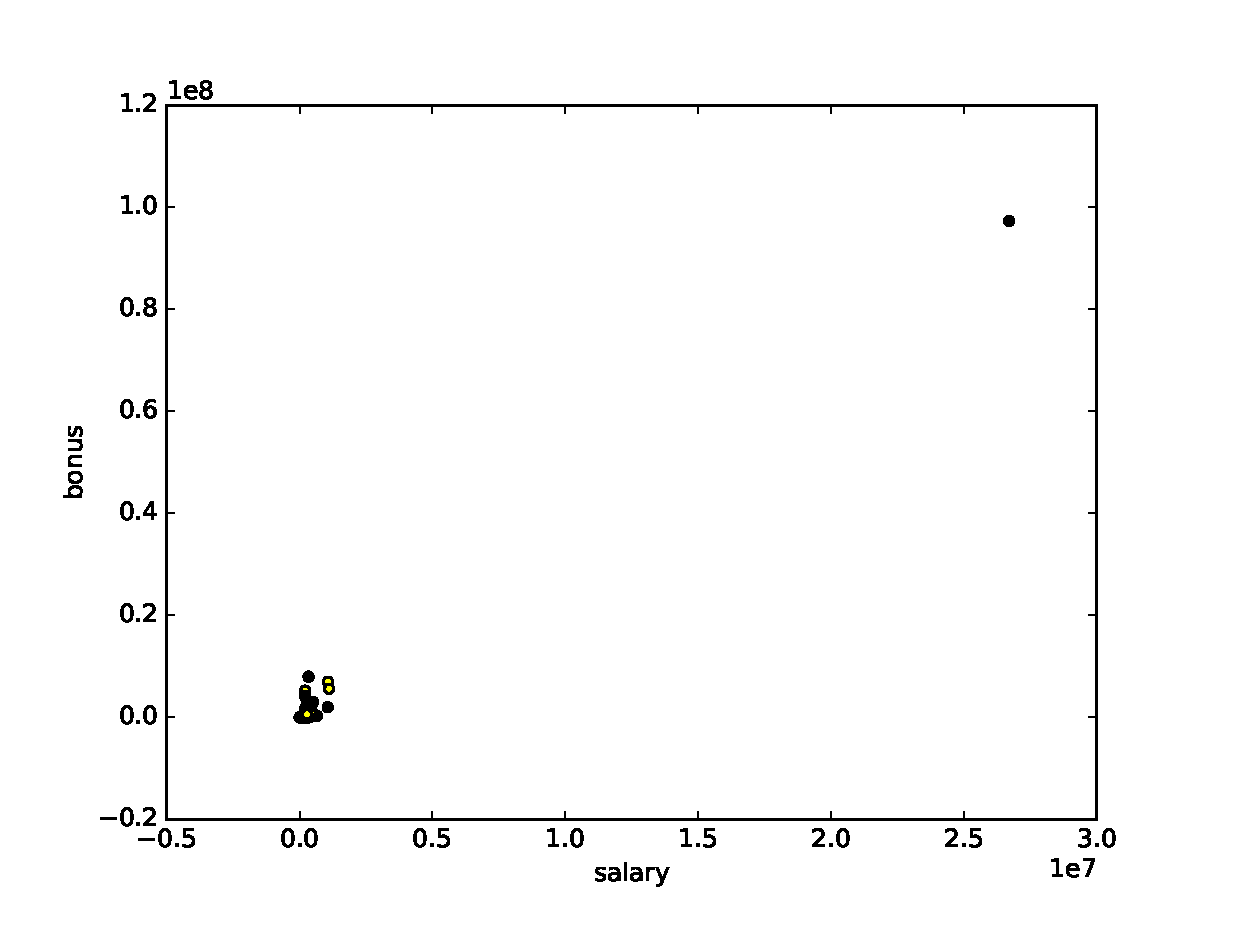
\includegraphics[width=1\textwidth]{outlier2.eps}}
  \hfill
  \subfloat[Data after outlier removal]{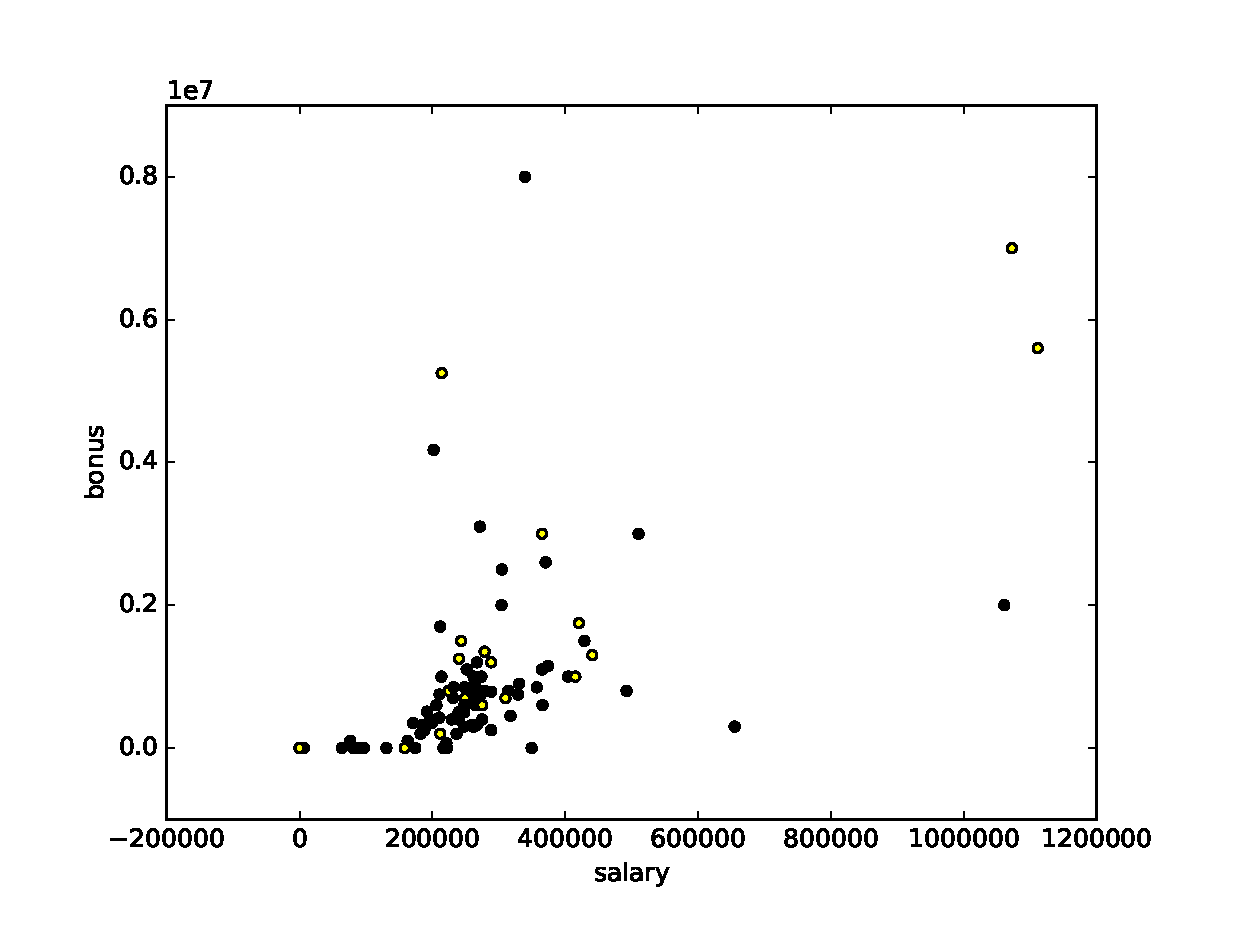
\includegraphics[width=1\textwidth]{notoutlier2.eps}}
  \caption{Salary vs bonus, POI's are marked in yellow}
\end{figure}

When looking at the completeness of each key, 'LOCKHART EUGENE E' was removed because it contained all 'NaN' values.
\\
\\
After the data was cleaned there were 143 records. These 143 records were used to create the machine learning predictive model. From the plots we can see that we have removed outliers and the data looks good for feature creation and use.

\newpage
\section*{Question 2}

What features did you end up using in your POI identifier, and what selection process did you use to pick them? Did you have to do any scaling? Why or why not? As part of the assignment, you should attempt to engineer your own feature that does not come ready-made in the dataset -- explain what feature you tried to make, and the rationale behind it. (You do not necessarily have to use it in the final analysis, only engineer and test it.) In your feature selection step, if you used an algorithm like a decision tree, please also give the feature importances of the features that you use, and if you used an automated feature selection function like SelectKBest, please report the feature scores and reasons for your choice of parameter values.

\subsection*{Solution}

\subsubsection*{Feature selection}
Firstly I had to look at the features one by one for POI and non POI in the data for completeness. As many data points in the data are 'NaNs' and carry no information looking at completeness is a good idea to select initial features to train the machine learning model.
The features we use to train the model to predict if a person is POI or not should contain enough information in both categories, hence carrying the information of a Non POI person too. Based on this reasoning the intial features I have used are
salary, bonus, deferral payments, deferred income, loan advances, long term incentive, restricted stock, total payments, total stock value, from messages, from poi to person, from person to poi and shared receipt with poi.

\newpage
\begin{table}[!htb]
\centering
\caption{Enron data completeness}
\label{my-label}
\begin{tabular}{lll}
 Features & POI completeness & Non POI completeness \\
 Bonus & .88 & .52 \\
 Salary & .94 & .62 \\
 Deferral payments & .28 & .26 \\
 Deferred income & .61 & .3 \\
 Director fees & 0 & .13 \\
 Exercised stock options & .67 & .71 \\
 Expenses & 1 & .60 \\
 From messages & .78 & .58 \\
 From poi to person & .78 & .58 \\
 From person to poi & .78 & .58 \\
 Loan advances & .05 & 0 \\
 Long term incentive & .67 & .42 \\
 Other & 1 & .58 \\
 Restricted stock & 1 & 1 \\
 Shared receipt with poi & .78 & .58 \\
 To messages & 0 & .13 \\
 Total payments & 1 & 1 \\
 Total stock value & 1 & 1 \\
 
\end{tabular}
\end{table}

Summarizing after cleaning up the data and removing outliers there are 143 people with features in the dataset of which 18 people are flagged as POI's, the rest are not POI's. Looking at the completeness of the data we can see that some features contain information on the POI and some do not, for example "Director fees" containes no information on the POI flagged data points and also carry very less information on the non POI side too. I did not use this feature in training the machine learning classifier. On the other hand "Restricted stock" in complete for both classes and is a useful feature.

\subsubsection*{Feature creation}

Using the the completeness of features I have selected the most consistence features to create more features to feed the machine learning classifier. This kind of feature creation will help the classifier predict better because it will contain all the information from the original features it was used to create.
\\
\\
The new features I created are as follows :

\begin{equation}
\mathrm{res\_total\_stock\_ratio} = \frac{\mathrm{restricted\_stock}}{\mathrm{total\_stock\_value}}
\end{equation}

\begin{equation}
\mathrm{salary\_total\_ratio} = \frac{\mathrm{salary}}{\mathrm{total\_payments}}
\end{equation}

\begin{equation}
\mathrm{bonus\_total\_ratio} = \frac{\mathrm{bonus}}{\mathrm{total\_payments}}
\end{equation}

\begin{equation}
\mathrm{from\_fraction\_messages} = \frac{\mathrm{from\_poi\_to\_this\_person}}{\mathrm{to_messages}}
\end{equation}

\begin{equation}
\mathrm{to\_fraction\_messages} = \frac{\mathrm{from\_this\_person\_to\_person}}{\mathrm{to\_messages}}
\end{equation}

\begin{equation}
\mathrm{salary\_bonus\_ratio} = \frac{\mathrm{salary}}{\mathrm{bonus}}
\end{equation}

Finally I will be using 20 features to train and test my classifiers and they are salary, bonus, deferral payments, deferred income, loan advances, long term incentive, restricted stock, total payments, total stock value, from messages, from poi to person, from person to poi, shared receipt with poi, restricted total stock ratio, salary total ratio, bonus total ratio, from fraction messages, to fraction messages, salary bonus ratio.
\\
\\
\newpage

\section*{Question 3}
What algorithm did you end up using? What other one(s) did you try? How did model performance differ between algorithms?  [relevant rubric item: “pick an algorithm”]

\subsection*{Solution}

Once we have decided on the features, lets now look at different classifiers and the performance of each with these features and data. I am using 'StratifiedShuffleSplit' to break the data into 1000 different train and test pairs. The performance index used for evaluating the classifier is 'f1 Score', 'precision score' and 'recall score'. We are using these metrics to evaluate the performance because accuracy score in this case is not a good way to evaluate the perforamce. We are looking for POI's in an unbalanced data set and using a metric that takes into acount the false positives and false negatives is more precise.

\begin{figure}[!htbp]
\centering
  \subfloat[With out MinMax scaling]{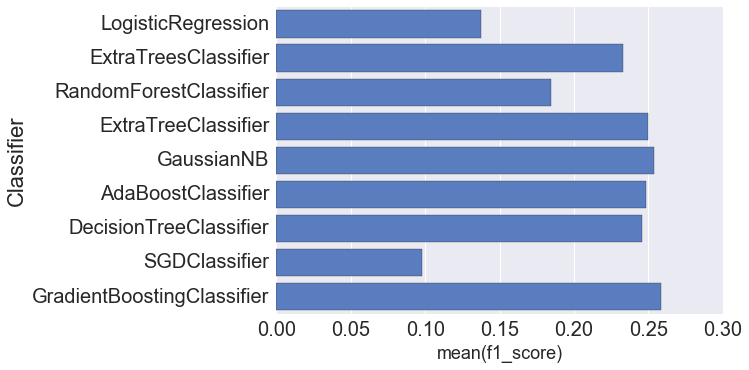
\includegraphics[width=1\textwidth]{notscale.png}}
  \hfill
  \subfloat[With MinMax scaling]{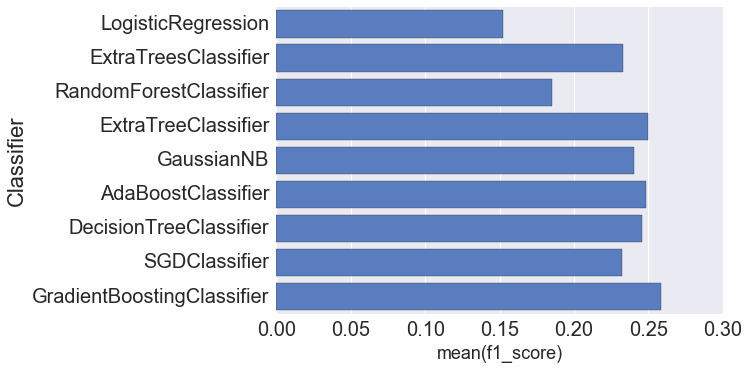
\includegraphics[width=1\textwidth]{scale.png}}
  \caption{Performance of different classifiers on the enron dataset}
\end{figure}

\begin{figure}[!htbp]
\centering
  \subfloat[With original features]{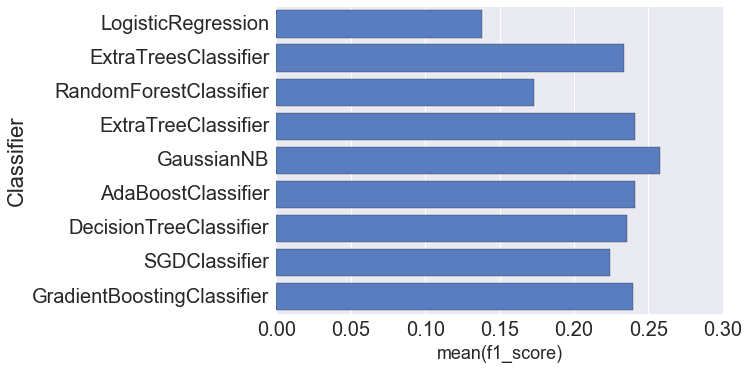
\includegraphics[width=1\textwidth]{class_image1.png}}
  \hfill
  \subfloat[With added features]{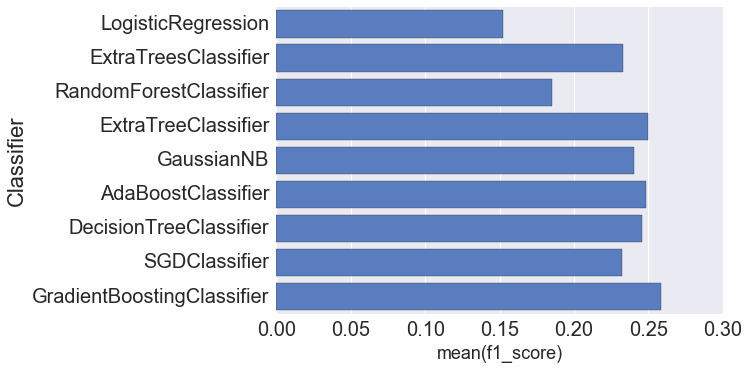
\includegraphics[width=1\textwidth]{class_image.png}}
  \caption{Performance of different classifiers on the MinMax scaled enron dataset}
\end{figure}

\begin{figure}[!htbp]
\centering
  \subfloat[Using a pipeline with scaling]{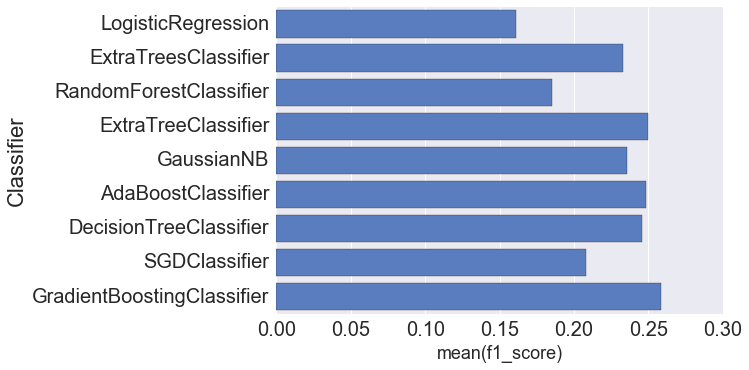
\includegraphics[width=1\textwidth]{pipelline.png}}
\end{figure}
\newpage
We can see that the classifiers performs better with added features and MinMax scaling. MinMax scaling is required because some of the data points vary a lot and scaling them to a number from 0 to 1 helps the classifier train better. The target is to choose a classifier to get a recall and precision score of 0.3. I will be using the Gradient Boosting Classifier to train and predict the POI's in the dataset. I personally like this classifier as it does not generally overfit the training data and performs better with test data.
\\
\\
Lets look at the importance of each feature in our Gradient boost classifier.
\begin{table}[!htb]
\centering
\caption{Enron data Gradient boost classifier feature importance}
\label{my-label}
\begin{tabular}{ll}
 Features & Importance \\
 Bonus & 0.16381 \\
 Salary & 0.02161 \\
 Deferral payments & 0.04275 \\
 Deferred income &  0.0222 \\
 Exercised stock options &  0.05072 \\
 Loan advances & 0.00029 \\
 Loag term incentive & 0.03419 \\
 Restricted stock & 0.09921\\
 Total payments & 0.07979 \\
 Total stock value & 0.12066 \\
 From messages & 0.02149 \\
 From poi to person & 0.03277 \\
 From person to poi &  0.00127 \\
 Restricted stock total ratio & 0.0410 \\
 Shared receipt with poi & 0.1087 \\
 To fraction messages & 0.05168 \\
 From fraction messages & 0.00312 \\
 Bonus total ratio & 0.0466 \\
 Salaray bonus ratio & 0.03 \\
 
\end{tabular}
\end{table}
\newpage
I performed a PCA transformation for the data and the performance of my classifier started to decrease hence I am not using PCA transformation.
\\
\\

%make importance table
\section*{Question 4}
What does it mean to tune the parameters of an algorithm, and what can happen if you don’t do this well?  How did you tune the parameters of your particular algorithm? (Some algorithms do not have parameters that you need to tune -- if this is the case for the one you picked, identify and briefly explain how you would have done it for the model that was not your final choice or a different model that does utilize parameter tuning, e.g. a decision tree classifier).  [relevant rubric item: “tune the algorithm”]

\subsection*{Solution}
Once we have decided on the classifier lets use grid search to tune the parameters of the classifier. Tuning the parameters of the algorithm means searching for values across a parameter grid for each feature and deciding which parameter to pass to the classifier based on a metric score. In this case 'f1 score' .
\\
\\
To decide which parameters to tune lets first see how the classifier performs with each parameter.


\begin{figure}[!htbp]
\centering
  \subfloat[Different parameters]{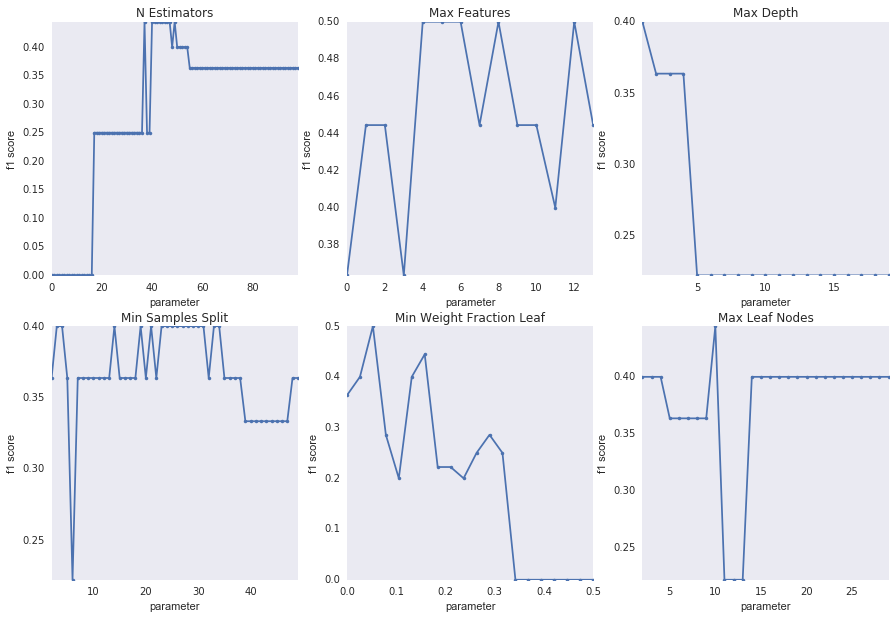
\includegraphics[width=1\textwidth]{3.png}}
  \caption{Performance of different parameters in the Gradient boost classifier on the enron dataset}
\end{figure}
We can see varying changes in the f1 score based on the feature grid. Now we can use the grid search from sklearn to decide what parameters will have the best f1 score on the test data.
\\
\\
If I had used an algorithm like the Gaussian naive bayes with no tunable parameters I would have used the SelectKBest to select the best features to train and changed the SelectKBest parameters to tune the algorithm.
\\
\\
If I do not hyper-tune my classifier then the performance of the classifier on a test or validation set will be poor. Its just a good way to generalize the classifier and improve its performance on data it has never seen.

The best tuned parameters are as follows:

\begin{table}[!htb]
\centering
\caption{Tuned parameter values of best performing gradient boost classifier}
\begin{tabular}{ll}
 Parameter & Value \\
 Max depth & 2 \\
 Max features & 3 \\
 Max leaf nodes & 2 \\
 Min samples leaf & 1 \\
 Min samples split & 3 \\
 Min weight fraction leaf & .05 \\
 N estimators & 4 \\
 Learning rate & 1 \\ 
 
\end{tabular}
\end{table}

\begin{table}[!htb]
\centering
\caption{Performance of gradient boost classifier before and after tuning }
\begin{tabular}{lllll}
 Classifier & accuracy & f1 score & precision & recall \\
 Before tuning & 0.85600 & 0.33002 & 0.43464 & 0.26600 \\
 After tuning & 0.87453 &  0.43313 & 0.54470 & 0.35950 \\ 
 
\end{tabular}
\end{table}


\section*{Question 5}
What is validation, and what’s a classic mistake you can make if you do it wrong? How did you validate your analysis?  [relevant rubric item: validation strategy]


\subsection*{Solution}

Validation is a process to train and test the machine learning algorithm based on a metric to access its performance, in this case performance can be computed by using accuracy score or the f1 score. If we do not perform validation properly then out machine learning algorithm might overfit the training data and end up performing poorly on the test data. We must validate our machine learning algorithm properly so it doesn't overfit the training data and performs optimally while running predictions unseen data.
\\
\\
I tried to validate using StratifiedShuffleSplit and GridsearchCV, but In this project the validation code was provided to me by Udacity. Its uses the StratifiedShuffleSplit in Scikit Learn with 1000 folds. This implementation was provided in the tester.py file.


\section*{Question 6}
Give at least 2 evaluation metrics and your average performance for each of them.  Explain an interpretation of your metrics that says something human-understandable about your algorithm’s performance. [relevant rubric item: “usage of evaluation metrics”]

\subsection*{Solution}

The evaluation metrics used to evaluate the performance with respect to the enron dataset is f1 score, precision score and recall score. We use these metrics because out data set in not balanced and using accuracy score will mislead us. We are trying to identify POI's and Non POI's in the data sets and using a metric that takes into account the false positives and false negatives in the way to go.
\\
\\
Here we define the metrics of evaluations as the following:

\begin{equation}
Precision = \frac{\mathrm{True\_positives}}{\mathrm{True\_positives} + \mathrm{False\_positives}}
\end{equation}

\begin{equation}
Recall = \frac{\mathrm{True\_positives}}{\mathrm{True\_positives} + \mathrm{False\_negatives}}
\end{equation}
\\
Precision is a measure of result relevancy, while recall is a measure of how many truly relevant results are returned. Hence we need optimal performance in both recall and precision of the classifier. For example a classifier with high precision and low recall will predict many labels correctly, but the majority of the positive predicted labels will be wrong. With respect to this dataset a low recall score means falsely identifying Non POI's as POI's which is not good.
\\
F1 score is defined as the following:
\begin{equation}
\mathrm{F1\_score} = 2 \times \frac{precision \times recall}{precision + recall}
\end{equation}
\\
The final performance of the classifier I chose are as follows:
\begin{table}[!htb]
\centering
\caption{Final performances of various classifiers after tuning	}
\begin{tabular}{lllll}
 Classifier & accuracy & f1 score & precision & recall \\
 GradientBoostingClassifier & 0.87453 &  0.43313 & 0.54470 & 0.35950 \\
 LogisticRegression & 0.79347 &  0.41613 & 0.33394 & 0.55200 \\
 ExtraTreesClassifier & 0.73640 &  0.40684  & 0.29061 & 0.67800 \\ 
 ExtraTreeClassifier & 0.80387 &  0.28093 & 0.30200 & 0.29108 \\
 AdaBoostClassifier & 0.85733 &  0.27849 & 0.42754 & 0.20650 \\
 GaussianNB & 0.79180 &  0.23996 & 0.24650 & 0.23376 \\
\end{tabular}
\end{table}
\\
\\
The tuned GradientBoostingClassifier \& LogisticRegression works well with the threshold set by the project, I chose to use GradientBoostingClassifier because of its higher f1 score.

\newpage
\section*{References}
\begin{itemize}
  \item \url{https://en.wikipedia.org/wiki/Enron_scandal	}
  
  \item \url{http://en.wikipedia.org/wiki/Enron_Corpus}

  \item \url{http://scikit-learn.org/stable/index.html} 
  
  \item \url{http://scikit-learn.org/stable/auto_examples/model_selection/plot_precision_recall.html}

  \item \url{http://scikit-learn.org/stable/modules/generated/sklearn.grid_search.GridSearchCV.html}
  
  \item \url{http://scikit-learn.org/stable/modules/generated/sklearn.ensemble.ExtraTreesClassifier.html}
  
  \item \url{http://scikit-learn.org/stable/modules/generated/sklearn.ensemble.RandomForestClassifier.html}
  
  \item \url{http://scikit-learn.org/stable/modules/generated/sklearn.feature_selection.SelectKBest.html}
  
  \item \url{http://scikit-learn.org/stable/modules/generated/sklearn.cross_validation.StratifiedShuffleSplit.html}
  
 \end{itemize}














\end{document}
